%!TEX root = virtual-clusters.tex

\section{Architecture} \label{S:architecture}

We provide a brief overview of the system architecture and summarize
the components which support user managed virtual HPC clusters in {\em
  Comet}.

\begin{figure}[!h]
  %\centering
\vspace{-.5cm}
   \hspace{-1.5cm} 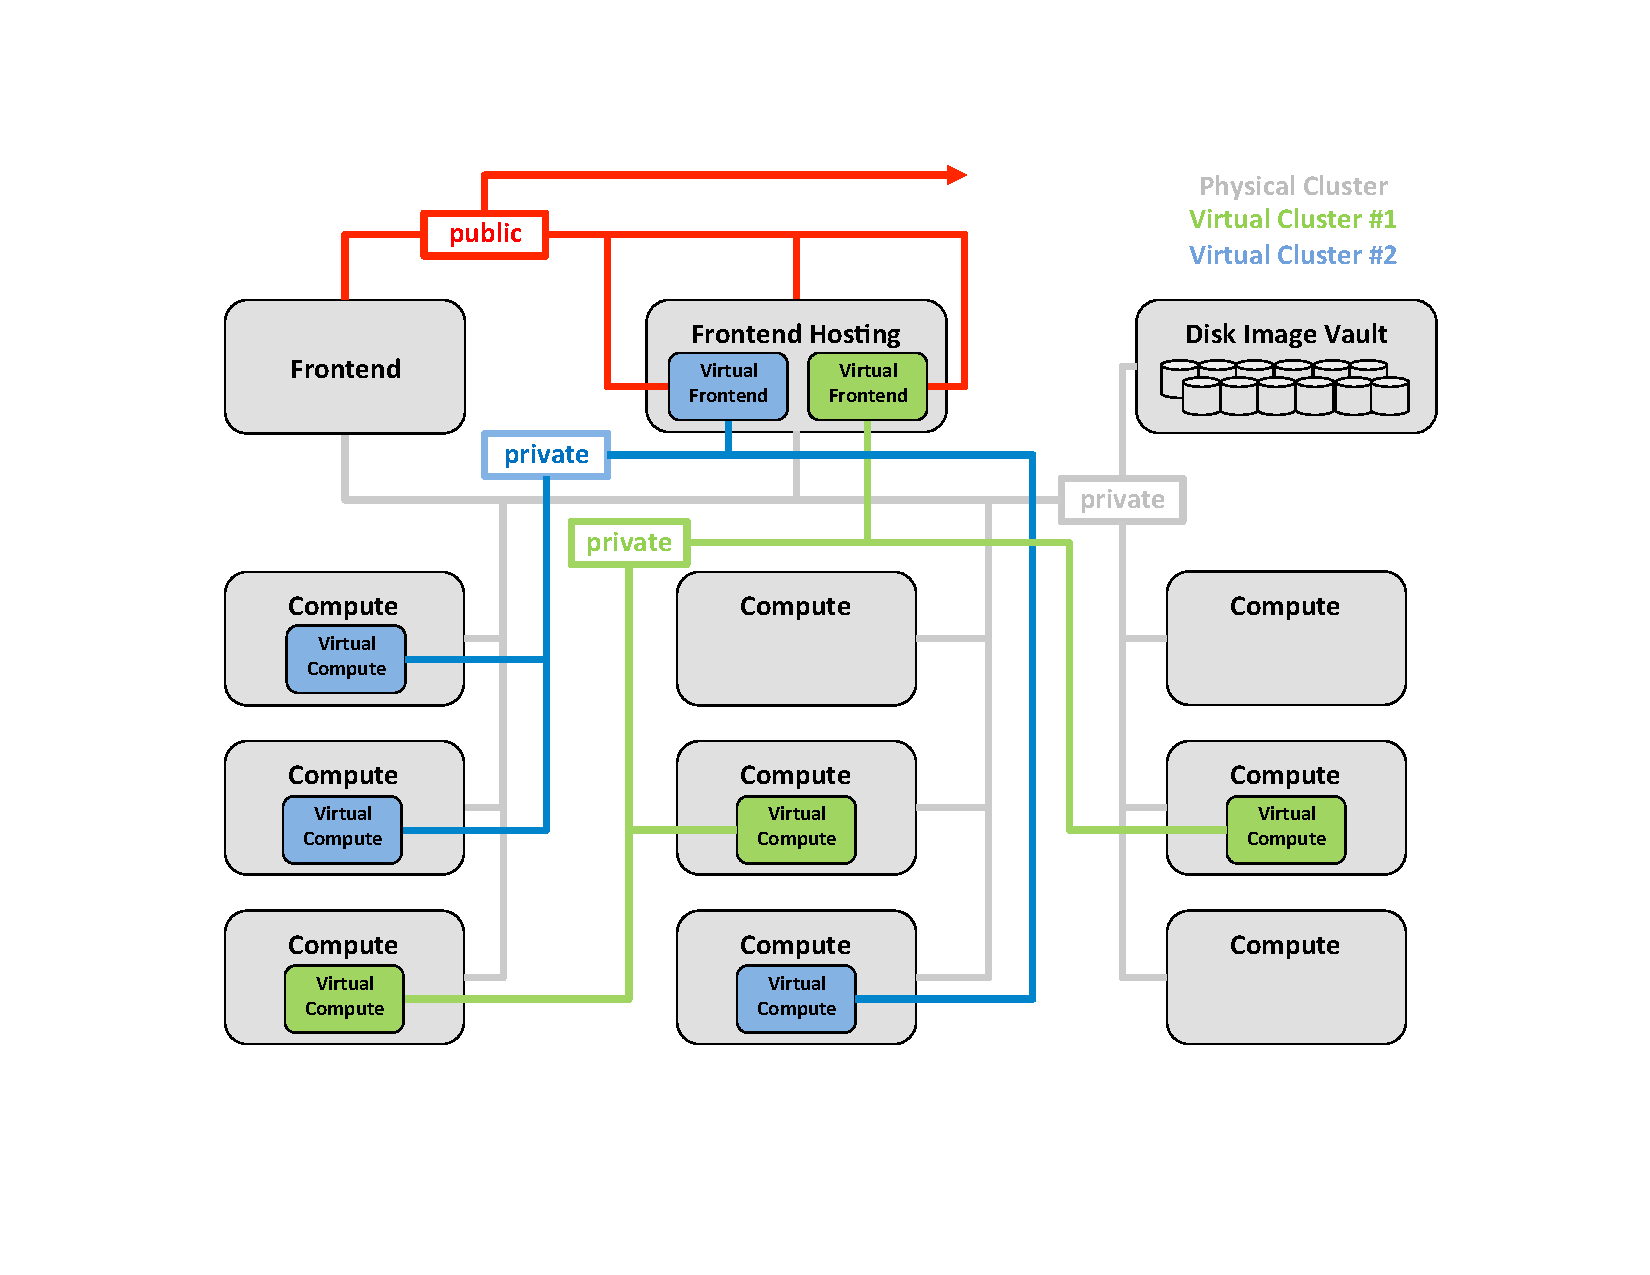
\includegraphics[width=1.3\columnwidth]{images/arch1}
\vspace{-1.5cm}

    \caption{Physical system architecture}
    \label{F:comet-arch1}
\end{figure}

{\parindent 0pt \bf Summary} The virtual cluster (VC) environment for {\em
Comet\/} is implemented largely on top of production HPC resources. {\em
Comet\/} standard compute nodes are used to host VC compute nodes (VCN) with
resource allocation managed by the production scheduler. The allocation of
standard compute nodes to the pool of nodes available for running VCNs can be
adjusted on demand.

Once a VC is defined on {\em Comet\/} a VC administrator is able to install the
VC frontend node (FN) with a system software management stack of their choice.
With the virtual FN installed and configured the VC administrator is able to start and
complete the installation and configuration of their VCNs. Installation of VCNs
can be interactive and manual or fully automated as all nodes can be PXE
installed inside the VC private network.

The resource usage of all VCNs is tracked as standard HPC jobs linked to
specific XSEDE allocations and usage is reported to XSEDE via the standard
mechanisms.

{\parindent 0pt \bf Nucleus.} The management platform we developed for this
coordination is called Nucleus and consists of a web service providing a REST API, a
database for maintaining state of managed resources, and a message queueing
system (based on RabbitMQ) providing connectivity and load balancing between
system components. Nucleus handles authentication and authorization of VC
administrators, tracks and orchestrates VCN state changes and resource
utilization, provides console access to the VC nodes using Guacamole
service. The state of VCNs is periodically pushed to the Nucleus management
database. The Nucleus database provides all needed information to VC
administrators requests for a state. The Nucleus database is ``eventually
consistent'' with the state of the physical cluster. This approach minimizes the
effect of VC administrator state requests on the production scheduler.

{\parindent 0pt \bf Rocks.} Rocks KVM roll provides the mechanism for running and
managing VMs on {\em Comet\/} physical hardware. Nucleus uses standard Rocks
commands to periodically query the state of all physical and virtual resources
and to execute commands on behalf of VC administrators to manage the resources
belonging to their VC.

\begin{figure}[!h]
  %\centering
\vspace{-.5cm}
     \hspace{-1.0cm} 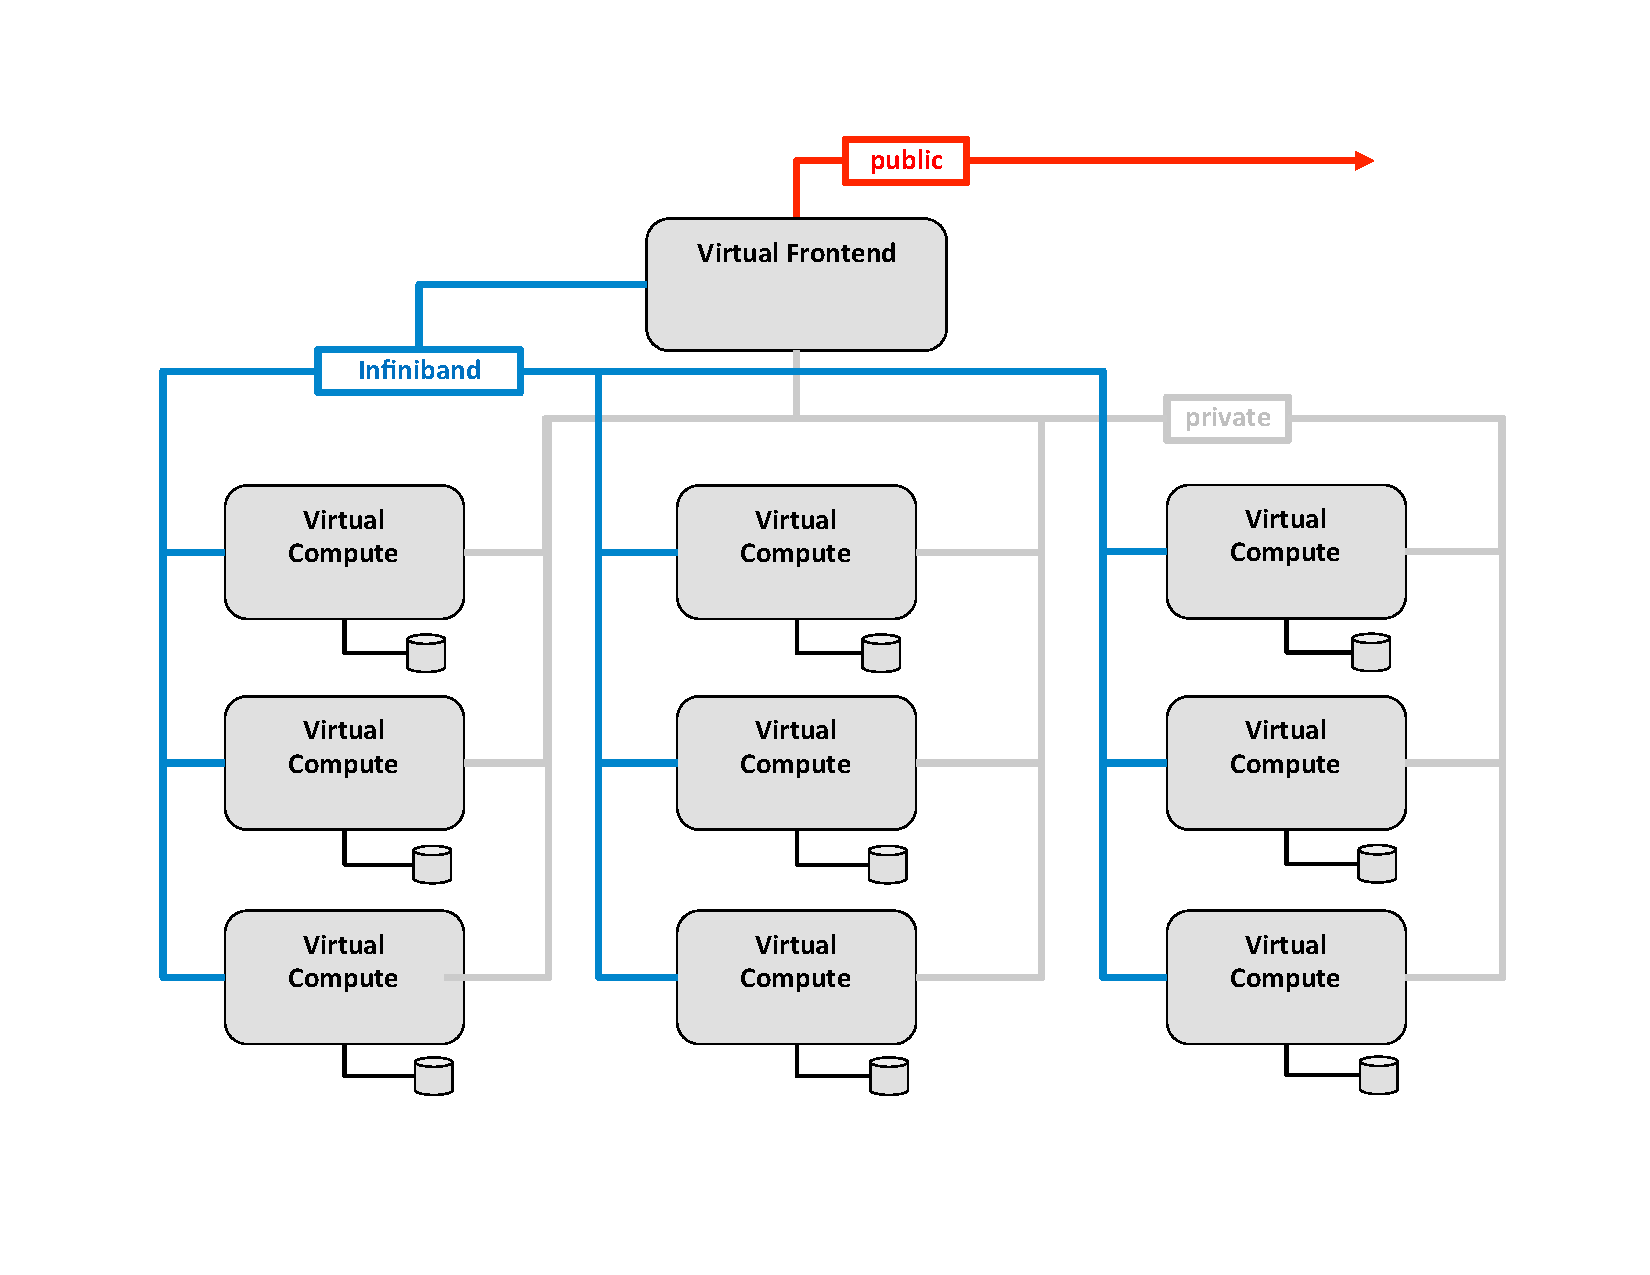
\includegraphics[width=1.2\columnwidth]{images/arch2}
\vspace{-1.5cm}
    \caption{Virtual cluster network topology}
\label{F:arch2}
\end{figure}

{\parindent 0pt \bf Networking.} Frontend and compute nodes are hosted on
physical hosts with two (private and public) or one (private) 10Gbps Ethernet
interfaces, respectively. The private network interfaces of all VMs in a VC are
connected to a logical VLAN device. Logical VLAN devices are raw, tagged packet
interfaces, using the Macvtap driver. Frontend public interfaces are bridged
either directly to a 10GbE interface or to a virtual VLAN device on the physical
host. Physical hosts also provide one FDR InfiniBand interface with one or more
Single Root IO Virtualization (SR-IOV) virtual functions enabled. All VMs of a
single VC are configured to use InfiniBand SR-IOV virtual functions with a
single common pkey.

{\parindent 0pt \bf Scheduling.} Frontend nodes run constantly at no charge and
provide access to the compute nodes of their associated virtual cluster. VC
administrators can start compute nodes on any physical compute node assigned by
the {\em Comet\/} scheduler.


%%% Local Variables:
%%% mode: latex
%%% TeX-master: t
%%% End:



\newcommand{\GET}{GET}
\newcommand{\DELETE}{DELETE}
\newcommand{\PUT}{PUT}
\newcommand{\POST}{POST}
\newcommand{\PATCH}{PATCH}


\begin{table*}[!h]
\caption{REST interface of the {\em Comet\/} virtual cluster service.}\label{T:rest}
\smallskip

\begin{small}
\begin{tabular}{|llp{6.5cm}|}
\hline
	& REST URL & Description \\
\hline
\GET	  & /v1/cluster/								     & gets the list of all clusters \\
\hline
\GET 	  & /v1/cluster/\{cluster.name\} 						     & Obtain details about the named cluster \\
\hline
\DELETE   & /v1/cluster/\{cluster.name\} 						     & Destroy the named cluster \\
\hline
\GET 	  & /v1/cluster/\{cluster.name\}/compute/\{compute.name\}		     & Obtain the details of a named compute resource  in a named cluster \\
\hline
\DELETE   & /v1/cluster/\{cluster.name\}/compute/\{compute.name\} 	      	     & Destroy the named compute resource in a  named cluster \\
\hline
\PUT 	  & /v1/cluster/\{cluster.name\}/compute/\{compute.name\}/attach        & iso Attach an ISO to the named compute resource in a named cluster   \\
\hline
\PUT 	  & /v1/cluster/\{cluster.name\}/compute/\{compute.name\}/poweroff      & Power off the named compute resource  in a named cluster \\
\hline
\PUT 	  & /v1/cluster/\{cluster.name\}/compute/\{compute.name\}/poweron 	     & Power on the named compute resource  in a named cluster \\
\hline
\PUT 	  & /v1/cluster/\{cluster.name\}/compute/\{compute.name\}/reboot 	     & Reboot the named compute resource in a  named cluster \\
\hline
\POST 	  & /v1/cluster/\{cluster.name\}/compute/\{compute.name\}/rename 	     & Rename the named compute resource  in a named cluster \\
\hline
\PUT 	  & /v1/cluster/\{cluster.name\}/compute/\{compute.name\}/reset 	     & Reset the named compute resource in a  named cluster \\
\hline
\PUT 	  & /v1/cluster/\{cluster.name\}/compute/\{compute.name\}/shutdown      & Shutdown the named compute resource in a named cluster  \\
\hline
\GET 	  & /v1/cluster/\{cluster.name\}/frontend/ 	     			     & Obtain the details of a frontend resource in a named cluster  \\
\hline
\PUT 	  & /v1/cluster/\{cluster.name\}/frontend/attach iso 			     & Attach an ISO to the frontendresource in a named cluster  \\
\hline
\PUT 	  & /v1/cluster/\{cluster.name\}/frontend/poweroff 		             & Power off the frontend of a named cluster  \\
\hline
\PUT 	  & /v1/cluster/\{cluster.name\}/frontend/poweron 			     & Power on the frontend of a named cluster  \\
\hline
\PUT 	  & /v1/cluster/\{cluster.name\}/frontend/reboot 			     & Reboot the frontend of a named cluster  \\
\hline
\PUT 	  & /v1/cluster/\{cluster.name\}/frontend/reset			     & Reset the frontend of a named cluster  \\
\hline
\PUT	  & /v1/cluster/\{cluster.name\}/frontend/shutdown 			     & Shutdown the frontend of a named cluster  \\
\hline
\GET 	  & /v1/cluster/\{cluster.name\}/compute/\{compute.name\}/console/  & Open VNC console to named  compute resource \\
\hline
\GET 	  & /v1/cluster/\{cluster.name\}/frontend/console/    	      		     & Open VNC console to name frontend resource  \\
\hline
\POST 	  & /v1/computeset/	  	  						     & Power on a set of computes creating a ComputeSet \\
\hline
\GET 	  & /v1/computeset/  								     & list the compute set \\
\hline
\GET 	   & /v1/computeset/\{computeset.id\} 						     & Obtain the details of the identified ComputeSet  \\
\hline
\PUT 	   & /v1/computeset/\{computeset.id\}/poweroff 					     & Power off the identified ComputeSet  \\
\hline
\PUT 	   & /v1/computeset/\{computeset.id\}/reboot					     & Reboot the nodes in the identified ComputeSet  \\
\hline
\PUT 	   & /v1/computeset/\{computeset.id\}/reset					     & Reset the nodes in the identified ComputeSet  \\
\hline
\PUT 	   & /v1/computeset/\{computeset.id\}/shutdown 					     & Shutdown the nodes in the identified ComputeSet  \\
\hline
\GET 	   & /v1/user 									     & Returns Users details in JSON format  \\
\hline
\PUT 	   & /v1/user 									     & Returns Users details in JSON format  \\
\hline
\PATCH 	   & /v1/user 									     & Returns Users details in JSON format  \\
\hline
\GET 	   & /v1/project 								     & Returns project details  \\
\hline
\GET 	   & /v1/image 								     & Gets the list of images  \\
\hline
\POST 	   & /v1/image 									     & Adds and image  \\
\hline
\end{tabular}
\end{small}


\end{table*}


{\parindent 0pt \bf Image Storage.} The implemtation of VCs in {\em Comet\/} also
requires a Network Attached Storage (NAS) (Disk Image Vault, Figure
\ref{F:comet-arch1}) --- a server with a large disk pool for VM images and ISO
files. VM images are stored as ZFS datasets on the NAS with each VM owning a
single image. The Image Storage system orchestrates the creation and destruction
of iSCSI targets providing read-only access to VM images resident on the NAS.
This allows VMs to start booting almost instantly. Image Storage also migrates a
copy of the VM image to the physical node hosting the VM and creates a local
temp-write volume to receive writes from the VM while the migration is underway.
After migration is complete the VM is briefly paused, the migrated VM image and
temp-write image are merged, the iSCSI target is disconnected and the VM is
resumed with both reads and writes accessing the local copy of the VM image.
At this point the VM is fully autonomous from the NAS providing great
capabilities of scaling without putting load on the NAS or network. Periodic
snapshots of the local, ZFS backed, VM images are automatically created and
copied back to the NAS keeping VM images backed up in case the physical node
crashes. The final synchronization of changes to VM images after VM shutdown
allows the VM image state to be persisted until the next VM boot.



{\parindent 0pt \bf Messaging.} We implemented an asynchronous communication
system between the components of the image management system, and also Nucleus
components connections using the AMQP messaging system RabbitMQ. We have Celery
workers running in several locations in the system, receiving AMQP messages with
jobs and normally replying with AMQP messages as well. This ensures smooth
operation under high loads by scheduling jobs in a queue rather than trying to
perform those as they come, and ease of scaling by adding more resources with
running daemons.

{\parindent 0pt \bf REST Interface}
In order to support the concept of virtual clusters on {\em Comet\/} we
provide a secure REST service to access them. The basic REST
signatures are listed in Table \ref{T:rest}. However the client
interface that uses these rest calls provide additional functionality
and allow easy scripting which is demanded by VC
administrators. We describe the client in Section \ref{S:cloudmesh}.

